\documentclass{beamer}
\usetheme{Rochester}
\usecolortheme{whale}
\usepackage[spanish,es-nodecimaldot]{babel}
\usepackage[utf8]{inputenc}
\usepackage[T1]{fontenc}
\usepackage{lmodern,amsmath,graphicx,float,color,booktabs,soul,mathrsfs}
\hypersetup{pdfstartview={Fit}}
\graphicspath{{./Img/}}
\usefonttheme[onlymath]{serif}

\title{El problema de la cuantización de la interacción gravitatoria}
\author{Iyán Méndez Veiga \and Víctor Rodríguez Bouza}
\date[TRG 2014/2015]

\begin{document}

\maketitle

\section{Introducción}
\subsection{Aproximación histórica}
\begin{frame}
\frametitle{Introducción}
\framesubtitle{Aproximación histórica}
\begin{itemize}
 \item Propuestas de Aristóteles y Ptolomeo.
 \item Revolución Científica del Renacimiento: \textbf{Copérnico} (s. XVII).
 \item \textbf{Kepler} (s. XVII): primer análisis físico de los cuerpos del sistema solar.
 \item \textbf{Newton} (s. XVII): primera concepción científica $\Rightarrow$ \textbf{Gravedad}
\end{itemize}
\end{frame}

\subsection{Gravedad newtoniana}
\begin{frame}
\frametitle{Introducción}
\framesubtitle{Gravedad newtoniana}
\begin{columns}[c]
  \begin{column}[c]{.5\textwidth}
  \begin{exampleblock}{Logros}
    \begin{itemize}
      \item Permitió entender la interacción de cuerpos diminutos y los más masivos.
      \item Interpretación de las leyes de Kepler.
      \item Descubrimiento de Nepturno.
    \end{itemize}
  \end{exampleblock}
  \begin{alertblock}{Problemas}
  \begin{itemize}
    \item No explica la precesión del perihelio de Mercurio.
  \end{itemize}
  \end{alertblock}
  \end{column}
  \begin{column}[c]{.5\textwidth}
    \centering
    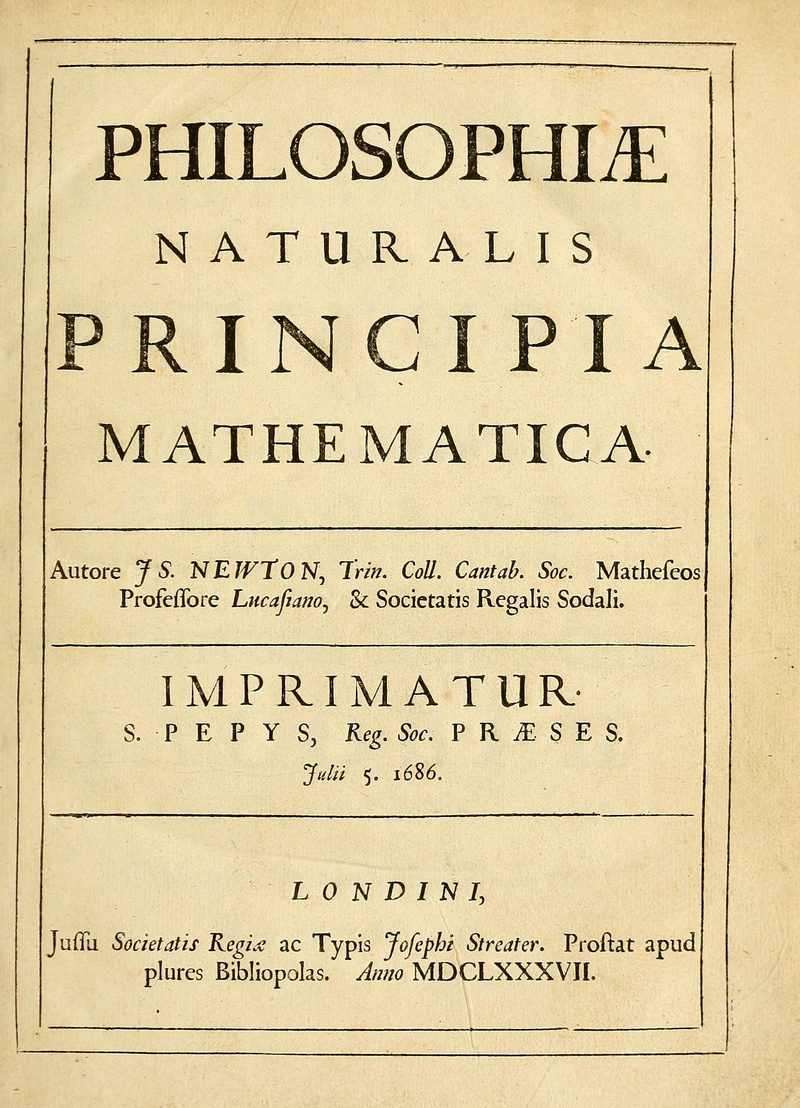
\includegraphics[height=4.5cm]{newton} \\
    {\small{\textit{Portada original de los} Philosophiae Naturalis Principia Mathematica\textit{ de Newton.}}}
  \end{column}
\end{columns}
\end{frame}

\subsection{Teoría de la Relatividad General}
\begin{frame}
\frametitle{Introducción}
\framesubtitle{Teoría de la Relatividad General}
\begin{columns}[c]
  \begin{column}{.5\textwidth}
    \centering
    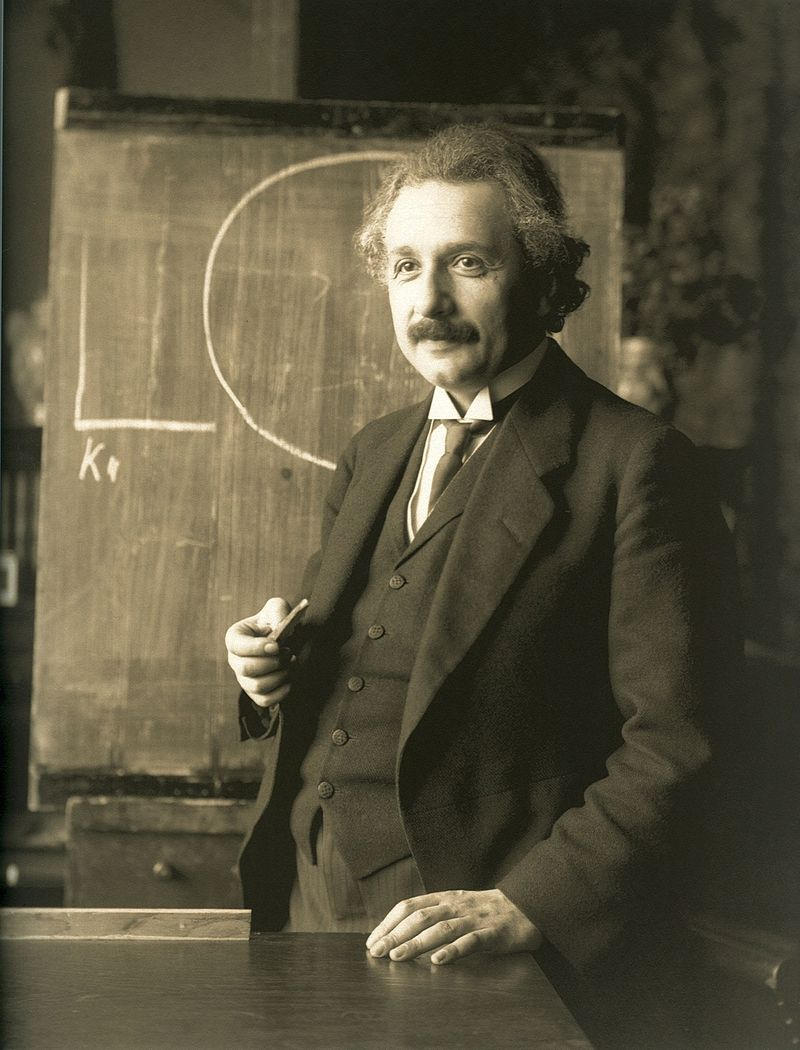
\includegraphics[height=5.5cm]{einstein} \\
    {\em\small Albert Einstein (1879-1955) fue uno de los más relevantes científicos del siglo XX.}
  \end{column}
  \begin{column}{.5\textwidth}
    \begin{itemize}
      \item La gravedad de Newton no era compatible con la Relatividad Especial.
      \item 10 años después de publicar la RE, Einstein publica un modelo no cuántico que incluye la RE y la gravedad newtoniana.
      \item Explica la precesión del perihelio de Mercurio y ha superado todos los test observacionales hasta la fecha (púlsares binarios).
    \end{itemize}
\end{column}
\end{columns}
\end{frame}

\section{Gravedad cuántica}
\subsection{¿Por qué es necesaria?}
\begin{frame}
\frametitle{Gravedad cuántica}
\framesubtitle{¿Por qué es necesaria?}
\begin{block}{}
  \begin{itemize}
    \item \textbf{Completitud formal}: búsqueda de una teoría \emph{superior}.
    \item \textbf{Unificación}
    \item \textbf{Singulariades} en RG: una teoría aún más general se espera que explique los agujeros negros, el Big Bang, \dots
    \item \textbf{El problema del tiempo}: tiempo absoluto de QM frente al tiempo dinámico de RG.
    \item \textbf{Incompletitud del modelo estándar}
  \end{itemize}
\end{block}
\end{frame}

\subsection{Los problemas de la cuantización}
\begin{frame}
\frametitle{Gravedad cuántica}
 \framesubtitle{Los problemas de la cuantización}
 \begin{exampleblock}{}
   \textbf{Renormalización}: procedimiento en el que se reajusta el lagrangiano del problema en función a unos parámetros de escala ($\alpha_{EM}$, $\alpha_{W}$...) para eliminar divergencias en los cálculos perturbativos.\\
   ~\\\centering
 Desarrollo perturbativo: $A=A_0\lambda^0+A_1\lambda^1+A_2\lambda^3+...$
\end{exampleblock}
 \begin{alertblock}{}
   La teoría cuántica perturbativa de la gravedad construida de forma análoga a QED es una \textbf{teoría no renormalizable}.
 \end{alertblock}
 \end{frame}

\subsection{¿Por dónde empezar?}
\begin{frame}
\frametitle{Gravedad cuántica}
\framesubtitle{¿Por dónde empezar?}
\begin{itemize}
  \item Los intentos de cuantizar la gravedad se suelen agrupar en \textbf{dos tipos}:
  \begin{enumerate}
    \item Punto de partida clásico (\textbf{RG} normalmente) + \textbf{Reglas de cuantización}
    \begin{itemize}
     \item Intentos covariantes (teoría de perturbaciones, integrales de camino...)
     \item Intentos canónicos (geometrodinámica, bucles...)
    \end{itemize}
    \item \textbf{Teorías unificadoras} de todas las interacciones (\textbf{teoría de cuerdas})
  \end{enumerate}
\end{itemize}
\end{frame}

\subsection{Gravedad cuántica covariante}
\begin{frame}
\frametitle{Gravedad cuántica covariante}
\begin{itemize}
  \item En los intentos covariantes se hace uso de la \textbf{covarianza cuadrimensional}.
  \item Hoy en día lo más habitual es utilizando la \textbf{integral de camino cuántica} usando el procedimiento de \textbf{Faddeev-Popov}
  \begin{equation*}
   Z[g]=\int\mathscr{D}g_{\mu\nu}(x)e^{iS[g_{\mu\nu}(x)]}
  \end{equation*}
  \item Teoría de perturbaciones (\textbf{reglas de Feynman})
  \begin{equation*}
  g_{\mu\nu}=\bar{g}_{\mu\nu}+\sqrt{32\pi G}f_{\mu\nu}
  \end{equation*}
  \item Aunque teoría similar al SM, \textbf{teoría no renormalizable} \\ $\Rightarrow$ \textbf{Teorías efectivas} (truncamientos)
\end{itemize}
\end{frame}

\subsection{Gravedad cuántica canónica}
\begin{frame}
\frametitle{Gravedad cuántica canónica}
\begin{itemize}
 \item El espacio-tiempo se \textbf{<<separa>>} en una familia de espacios parametrizada por un único parámetro $t$. \\$\Rightarrow$ Espacio-tiempo $\equiv$ Trayectoria de espacios tridimensionales.
 \item Ahora se pueden plantear \textbf{problemas de valor inicial} a las ecuaciiones de Einstein. ¿Cómo evoluciona nuestra variedad a lo largo del <<tiempo>>?
 \item Con este formalismo surgen unas \textbf{ligaduras (clásicas)} conectadas con las invariancias de la teoría ($\mathscr{H}_\perp$, $\mathscr{H}_a$).
 \item La teoría cuántica de la gravedad se obtiene \textbf{cuantizando estas ligaduras}.
\end{itemize}
\end{frame}


\subsubsection{Geometrodinámica}
\begin{frame}
\frametitle{Gravedad cuántica canónica}
\framesubtitle{Geometrodinámica}
\begin{itemize}
 \item Introducida por Arnowitt, Deser y Misner (formalismo ADM) en los \textbf{años 60}, y muy promovida por \textbf{John Wheeler}.
\end{itemize}
\begin{align*}
  \mathscr{H}_\perp\Psi\equiv\Big(-16\pi G\hbar^2G_{\mu\nu\sigma\tau}\frac{\delta^2}{\delta g_{\mu\nu}\delta g_{\sigma\tau}}-\frac{\sqrt{g}}{16\pi G}(R-2\Lambda)\Big)\Psi&=0\\
 \mathscr{H}_a\Psi\equiv-2D_\nu h_{\mu\sigma}\frac{\hbar}{i}\frac{\delta\Psi}{\delta g_{\nu\tau}}&=0\,,
\end{align*}
\begin{itemize}
 \item Wheeler quería reducir toda la física a la \textbf{geometría} del espacio-tiempo. La dinámica de la geometría explicaría la masa, la carga y los campos $\Rightarrow$ \emph{\textbf{geons}}
\end{itemize}
\end{frame}

\subsubsection{Gravedad cuántica de bucles}
\begin{frame}
\frametitle{Gravedad cuántica canónica}
\framesubtitle{Loop Quantum Gravity}
\begin{itemize}
 \item El punto de partida son \textbf{teorías de gauge} basadas en los grupos espcial unitarios $SU(N)$.
 \item El propio \textbf{espacio está cuantizado} (espacio granulado)\\$\Rightarrow$ Tejido de lazos finitos (\emph{loops})
 \item Se estudia la evolución de las \textbf{redes de espín} con el tiempo (\emph{spin foam}).
 \item Es uno de los intentos de cuantizar la gravedad en el que más se investiga.
 \item \textbf{No pretende una gran unificación} basándose en alguna simetría más general, <<sólo>> aspira a cuantizar la teoría de Einstein en cuatro dimensiones.
\end{itemize}
\end{frame}
%
%
\section{Teoría de cuerdas}
\begin{frame}
  \frametitle{Teoría de cuerdas}
  \begin{block}{Orígenes}
    \begin{itemize}
      \item Grupo de trabajo iniciado por Werner Heisenberg (\textbf{1943}) $\Rightarrow$ \textit{S-matrix theory}.
      \item Formalmente, desde los \textbf{años sesenta}.
    \end{itemize}
  \end{block}
  \begin{block}{Qué es la teoría de cuerdas}
    \begin{itemize}
      \item \textbf{Nuevo marco teórico general}. No parte de soluciones existentes para resolver el problema. La gravedad cuántica aparece como resultado natural.
      \item Basada en el concepto de \textbf{cuerda}: nuevo ente elemental unidimensional que está definida en un espacio de más de cuatro dimensiones.
    \end{itemize}
  \end{block}
\end{frame}
%
%
\begin{frame}
  \frametitle{Teoría de cuerdas}
  \begin{exampleblock}{Aportaciones de la teoría de cuerdas}
    \begin{itemize}
      \item Plausible marco teórico general, \textbf{candidata} (discutida) \textbf{a TOE}.
      \item \textbf{Nuevas \textit{ideas} aplicables} no sólo a la propia teoría, sino también \textbf{a otros campos} (p. ej.: materia condensada).
    \end{itemize}
  \end{exampleblock}
  \begin{alertblock}{Problemas}
    \begin{itemize}
      \item \textbf{No es \textit{background independent}} (con la excepción de un caso parcial bajo AdS/CFT).
      \item \textbf{Carece de predicciones que puedan ser comprobadas experimentalmente en la actualidad}: la gran discordia de \textit{string theory}.
    \end{itemize}
  \end{alertblock}
\end{frame}
%
%
\section{Teorías de campo efectivas}
\begin{frame}
\frametitle{Teorías de campo efectivas}
\begin{block}{Qué son}
  \begin{itemize}
    \item Se basan en \textbf{conseguir resultados aproximados} para un intervalo de energías determinado.
    \item No tratan de resolver el problema de forma global.
    \item En los últimos años están recibiendo mayor impulso.
  \end{itemize}
\end{block}
\end{frame}
%
%
\begin{frame}
\frametitle{Teorías de campo efectivas}
\begin{exampleblock}{Ventajas}
  \begin{itemize}
    \item No necesitan que la teoría sea renormalizable para aplicarse.
    \item No son exclusivas de la gravitación: usadas en otros campos con éxito (p. ej.: materia condensada o física de partículas).
    \item Posible futuro prometedor en la cosmología cuántica.
  \end{itemize}
\end{exampleblock}
\begin{alertblock}{Problemas}
  \begin{itemize}
    \item \textbf{No están desarrolladas en totalidad}, aunque existen cálculos y predicciones experimentales...
    \item ...pero están lejos de las precisiones que nuestros instrumentos pueden medir.
  \end{itemize}
\end{alertblock}
\end{frame}
%
%
\section{Otras aproximaciones}
\begin{frame}
\frametitle{Otras aproximaciones}
\begin{block}{Teoría de sistemas causales fermiónicos}
  \begin{itemize}
    \item Procede de QFT y consiste en llegar a la relatividad general desde un sistema causal de fermiones.
  \end{itemize}
\end{block}
\begin{block}{Gravedad cuántica euclidiana}
  \begin{itemize}
    \item Esta aproximación trata de acceder a la gravitación cuántica usando un método de resolver problemas basado en la rotación de Wick: una transformación que permite hacer el cambio $d=n \rightarrow d=n+1$.
  \end{itemize}
\end{block}
\end{frame}
%
%
\begin{frame}
\frametitle{Otras aproximaciones}
\begin{block}{Teoría de tuistores (\textit{twistor theory})}
  \begin{itemize}
    \item Generalización de la teoría de espinores de Dirac de QFT que emplea números complejos para introducir Minkovski de 3+1 en un espacio 4-dimensional particular.
    \item Aplicada a \textit{Quantum Loop Theory} y teoría de cuerdas.
  \end{itemize}
\end{block}
\begin{block}{Teoría del vacío de superfluido}
  \begin{itemize}
    \item Reinterpreta el vacío como superfluido o condensado de Bose-Einstein.
  \end{itemize}
\end{block}
\begin{block}{Aproximaciones tangenciales: la métrica acústica}
  \begin{itemize}
    \item Las singularidades son similares a las de un agujero negro.
  \end{itemize}
\end{block}
\end{frame}
%
%
\section{Cosmología cuántica}
\begin{frame}
\frametitle{Cosmología cuántica}
\begin{itemize}
 \item Una de las aplicaciones de las teorías cuánticas de la gravedad para estudiar el \textbf{universo como un todo}.
 \item Problema de formular la teoría cuántica para un \textbf{sistema cerrado desde dentro de él} sin observadores externos ni mediciones.
 \item Tantas formulaciones como formulaciones de la gravedad cuántica.
 \item Ecuaciones diferenciales difíciles de resolver $\Rightarrow$ Teorías efectivas.
 \item Muchas de las características de la cosmología cuántica se estudian en el límite WKB.
\end{itemize}
\end{frame}

\section{Conclusiones}
\begin{frame}
\frametitle{Conclusiones}
\begin{block}{}
  \begin{itemize}
    \item Las pruebas experimentales más recientes confirman las predicciones de la relatividad general y de la física cuántica (\textit{p. ej., púlsares binarios}).
    \item Existen razones para buscar la cuantización de la gravedad.
  \end{itemize}
\end{block}
\begin{alertblock}{¿Qué problemas hay para hallarla?}
  $\Rightarrow$ Falta de resultados experimentales por limitaciones tecnológicas.
\end{alertblock}
\end{frame}

\begin{frame}
  \frametitle{Conclusiones}
  \begin{exampleblock}{Perspectivas futuras.}
    \begin{itemize}
      \item Nuevos telescopios e instrumentos que permitan medidas experimentales mejores (SNAP, Euclid, ALMA...).
      \item Desarrollo de nuevos campos y aproximaciones teóricas: cosmología cuántica, teorías efectivas...
      \item No se espera una resolución inmediata del problema (\textit{¿quizás se necesite una «mente brillante»?}).
    \end{itemize}
  \end{exampleblock}
  \centering
  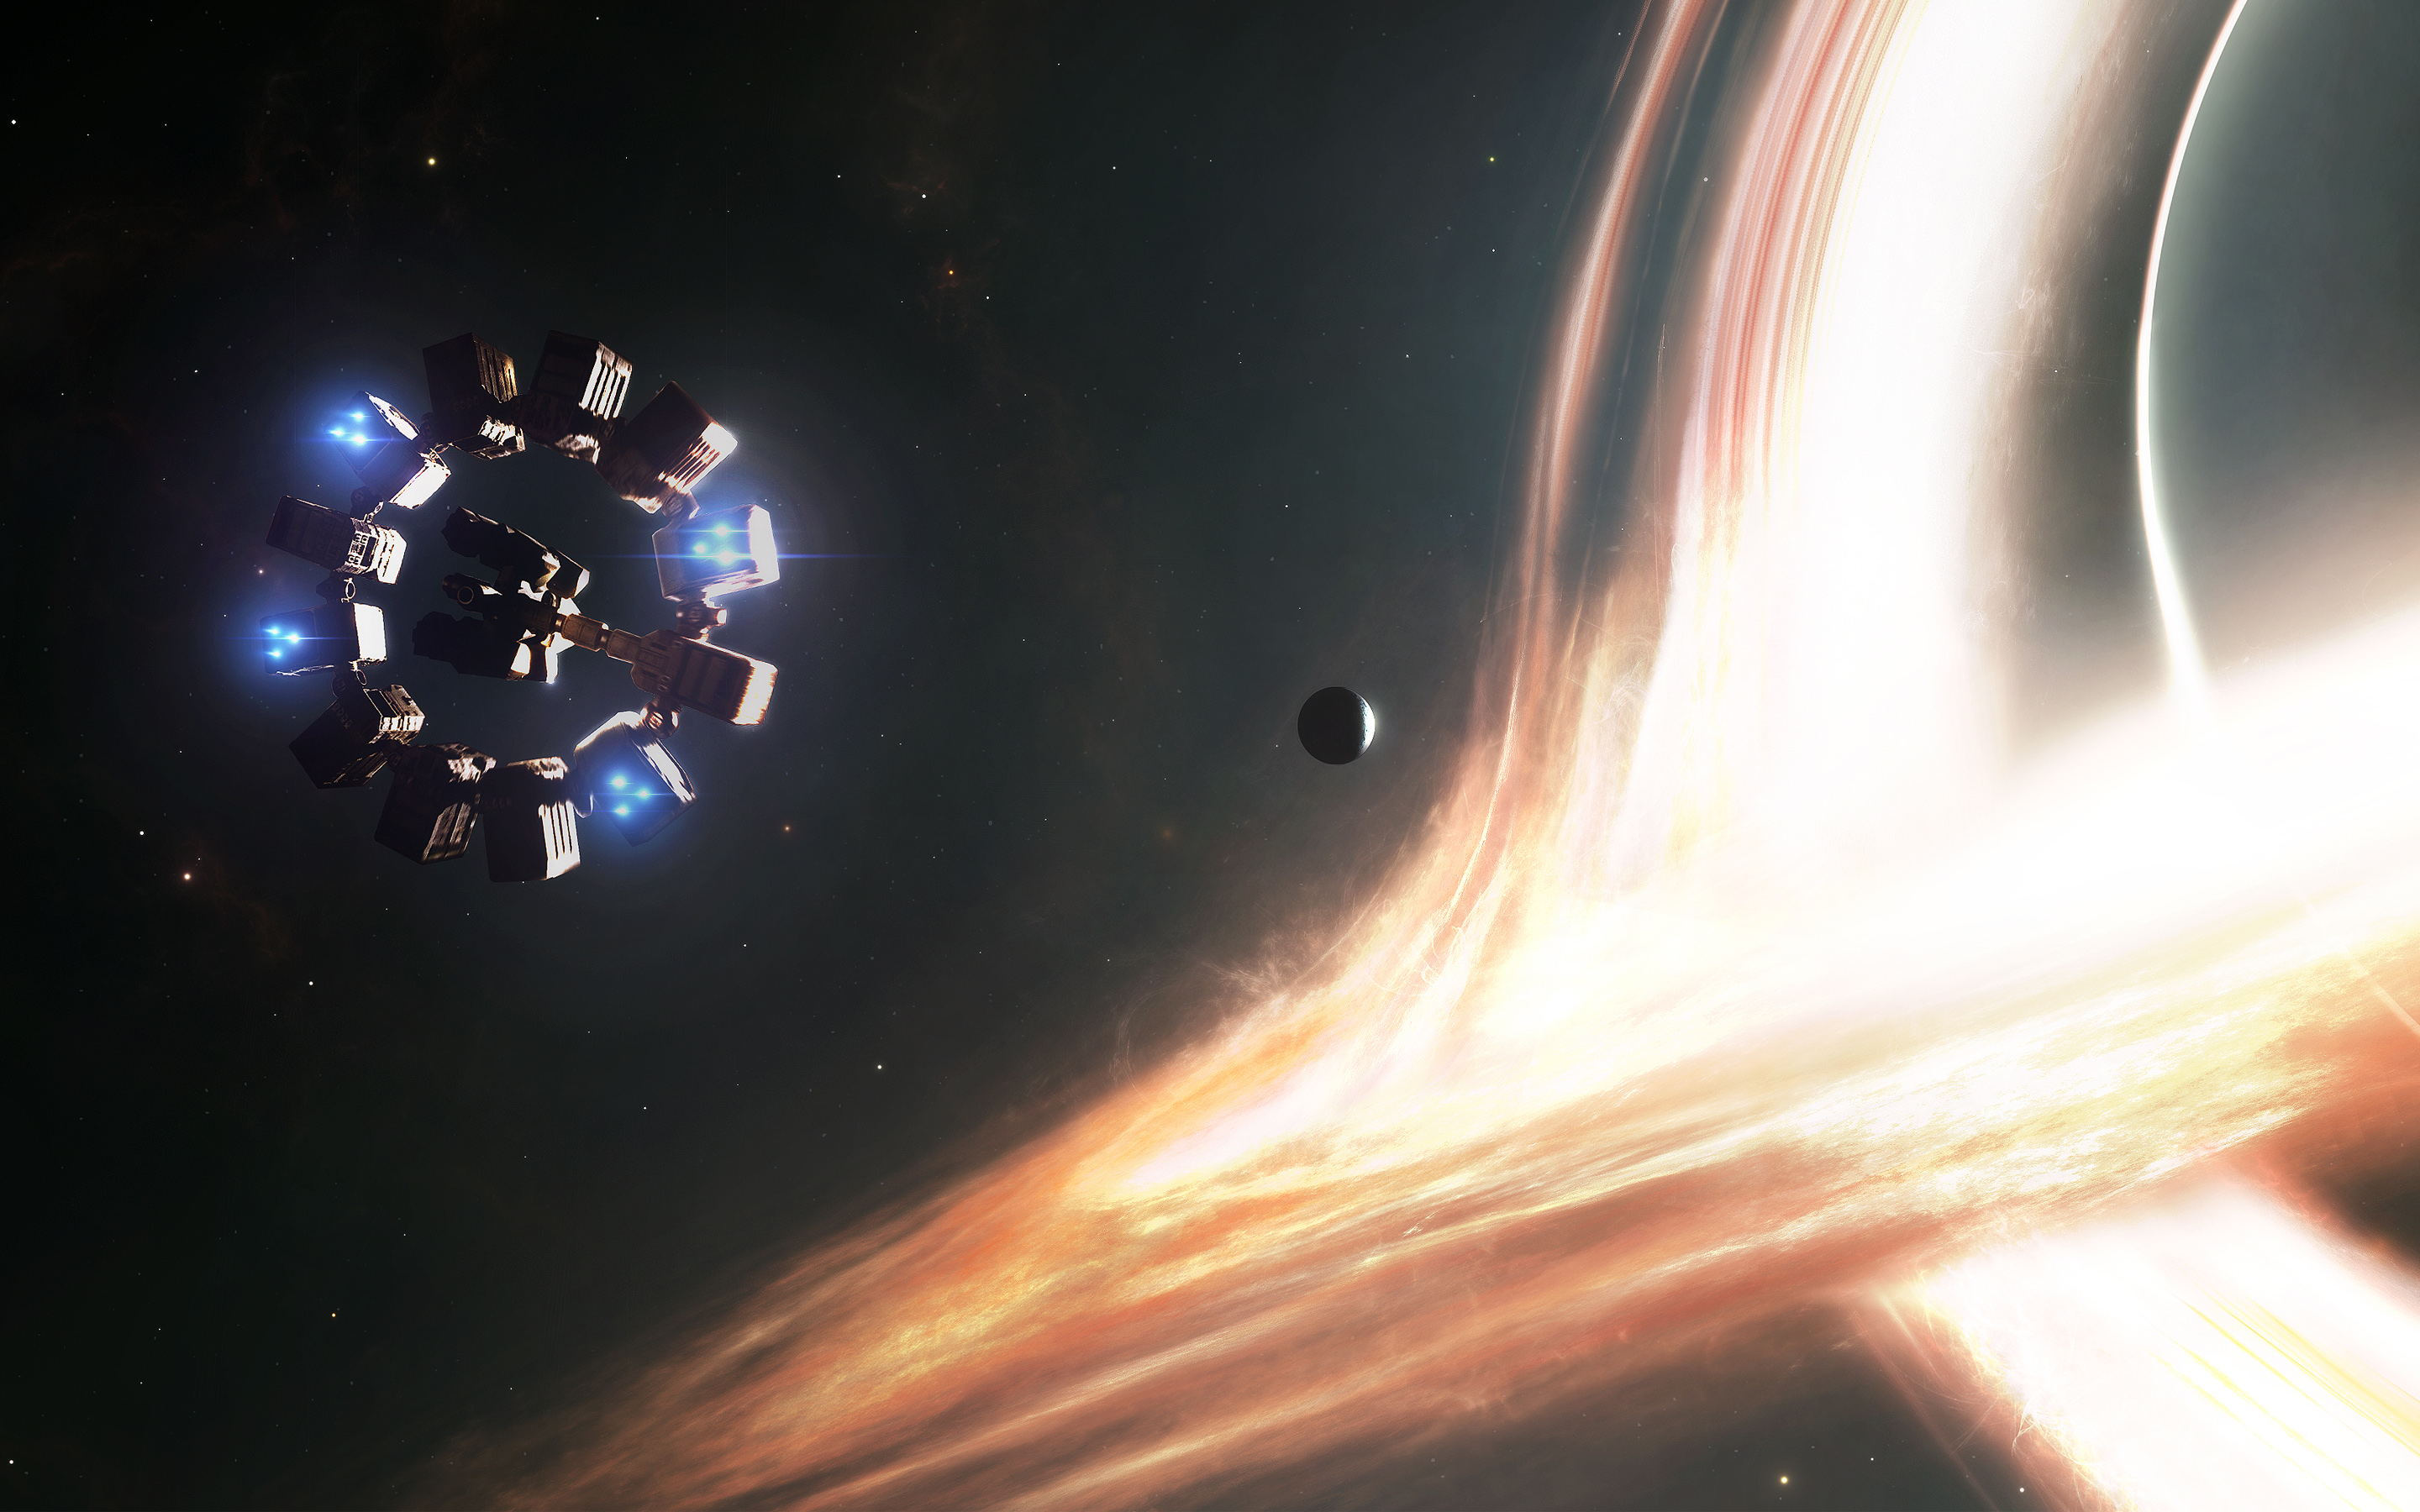
\includegraphics[width=.4\textwidth]{interstellar2} \\
  {\em\small El universo: la última frontera.}
\end{frame}


\begin{frame}[allowframebreaks]
  \frametitle<presentation>{Bibliografía}
  \begin{thebibliography}{10}
  \beamertemplatebookbibitems
  \bibitem{lib:Ferreira}
    P.G.~Ferreira.
    \newblock {\em La teoría perfecta - Un siglo de figuras geniales y de pugnas por la teoría general de la relatividad}.
    \newblock Editorial Anagrama (Colección Argumentos), 1ed, 2015.
  \beamertemplatearticlebibitems
  \bibitem{art:Kiefer}
    C.~Kiefer.
    \newblock {\em Conceptual problems in quantum gravity and quantum cosmology}.
    \newblock Mathematical Physics, p. 17, 2013.
  \bibitem{art:Guilini}
    D.~Guilini y C.~Kiefer.
    \newblock {\em The canonical approach to quantum gravity: general ideas and geometrodynamics}.
    \newblock p. 21, 2006
  \bibitem{art:Lijing}
    S.~Lijing {\em et all}.
    \newblock {\em Testing gravity with pulsars in the SKA era}, 2015.
  \bibitem{art:Anderson}
    P.R.~Anderson y D.R.~Brill.
    \newblock {\em Gravitational geons revisited}.
    \newblock Physical Review D, vol. 56, 1997.
  \bibitem{art:Burgess}
    C.P.~Burgess
    \newblock {\em Quantum gravity in everydan life: general relativity as an effective field theory}.
    \newblock Living Reviews in Relativity, vol. 7, p. 5, 2004.
  \end{thebibliography}
\end{frame}

\end{document}
